\scanpage{63}
\[
[p(\overline F)\subset p(\overline F')]\Longleftrightarrow\overline F\subset\overline F'
\]

\figure{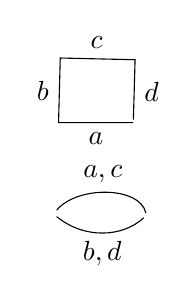
\begin{tikzpicture}[x=0.72cm,y=0.72cm,line cap=round]
\draw (1.32,.06)--(1.35,1.11)--(.03,1.14)--(0,0)--(1.31,0);
\node[below] at (.66,0) {$a$}; \node[left] at (0,.56) {$b$};
\node[above] at (.67,1.13) {$c$}; \node[right] at (1.34,.55) {$d$};
\draw (-.03,-1.54) .. controls (.33,-1.11) and (1.43,-1.12) .. (1.54,-1.59);
\draw (-.03,-1.66) .. controls (.45,-2.05) and (1.12,-2.03) .. (1.5,-1.68);
\node[above] at (.78,-1.23) {$a,c$}; \node[below] at (.77,-1.92) {$b,d$};
\end{tikzpicture}}

\uline{NB} On trouve une décomposition de $P(E)$ \deleted{\unsure{en}} en parties qui sont des cellules top -- les intersections entre deux telles cellules, si elles sont non vides, étant une cellule ou réunion de 2 cellules disjointes (donc ce n'est pas tjrs une cellule) Le schéma combinatoire de cette division cellulaire (ens ordonné des parties envisagées) est \deleted{\unsure{le}} $\Phi^{**}/\sigma\simeq$ ensemble ordonné opposé de $\unsure{\Psi^*|\Psi^\times|\Phi^*}/\sigma$, où $\Psi^*$ \unsure{est|$\to$} l'ens des sections partielles non vides de $B$ sur $I$.

Automorphismes des cubes gauches $(n\geq3)$
\[
\operatorname{Aut}(C)/\sigma\xrightarrow{\sim}\operatorname{Aut}_{\mathrm{proj}}\widetilde C\xrightarrow{\sim}\operatorname{Aut}_{\mathrm{ord}}(\Phi(\widetilde C))\qquad ?
\]

On sait déjà que la première \unsure{appliction|application} est injective, il est évident que la seconde l'est, le composé \deleted{\unsure{S|est}} est \deleted{\unsure{aussi}} surjectif ?

Si $n$ impair, on récupère $(\unsure{\mathcal X|\partial C|X|\mathcal H},\sigma)$ avec division cellulaire comme le rev. orienté canonique de $\widetilde C$, et tt autom de $\Phi(\widetilde C)$ est induit par un autom orienté de $\widetilde C$. Cas $n$ pair : à examiner \ldots
% archive sheet number: 62
